\section*{Question 2}

\subsection*{Newton-Raphson}
Soit la fonction $G$ de la question 1. On souhaite appliquer la méthode de Newton pour trouver le point $s$ tel que $G(s)=0$. On a montré précédemment que $G(y)=0$ si  $(w+ W_{\bot}y)$ est un vecteur propre de $A$. On va maintenant montrer que cela est également vrai dans l'autre sens : lorsque $G(y)=0$, alors $(w+ W_{\bot}y)$ est un vecteur propre de $A$. On va montrer que $G(y)=0 \Rightarrow (w+W_{\bot}y)$ est vecteur propre de $A$.\\
On part du principe que $G(y)=0$, c'est-à-dire :
$$W_{\bot}^*A(w+W_{\bot}y)=w^*A(w+W_{\bot}y)y$$
On pose $A(w+W_{\bot}y) = \alpha (w+W_{\bot}y) + v$ où $v$ est orthogonal à $(w+W_{\bot}y)$ et $\alpha$ est un scalaire quelconque\footnote{De manière générale, $A(w+W_{\bot}y)$ renvoie un vecteur quelconque avec une composante parallèle à $w+W_{\bot}y$ et une composante orthogonale à ce même vecteur.}. L'équation ci-dessus devient alors $$W_{\bot}^*\alpha(w+W_{\bot}y)+W_{\bot}^*v=w^*\alpha(w+W_{\bot}y)y+w^*vy.$$
On a déjà montré dans la première question que $W_{\bot}^*\alpha(w+W_{\bot}y)=w^*\alpha(w+W_{\bot}y)y$. L'équation devient alors $$W_{\bot}^*v=w^*vy.$$
On a alors les deux relations suivantes :
$$(w^*+y^*W_{\bot}^*)v=0 \Leftrightarrow -y^*W_{\bot}^*v = w^*v \text{ (orthogonalité)}$$
et
$$W_{\bot}^*v=w^*vy.$$
En utilisant les deux équations ci-dessus, on trouve
$$y^*w^*vy+w^*v=0 \Leftrightarrow w^*v(y^*y+1)=0.$$
Ceci implique que la vecteur $v$ est nul et que, par conséquent, $w+ W_{\bot}y$ est vecteur propre de $A$\footnote{On pourrait également avoir $w^*v=0$ avec $v$ non nul mais cela impliquerait $W_{\bot}y=0$ et donc $y=0$. Dans ce cas, l'équation deviendrait $W_{\bot}^*Aw=0$ ce qui implique que $w+W_{\bot}y$ est vecteur propre de A (associé à la valeur propre $0$).}. Cela est très utile car on sait maintenant que la méthode de Newton appliquée à $G$ permet donc bien de trouver les vecteurs propres de $A$.

Nous allons maintenant nous intéresser à la convergence de cette méthode. Dans notre cas, on voit aisément que $G$ est dérivable que sa jacobienne $J_G(y) = W_{\bot}^*AW_{\bot} - w^*AwI - (yw^*AW_{\bot}+Iw^*AW_{\bot}y)$ est continue en $s$ tel que $G(s)=0$ ($I$ est la matrice identité de taille $n-1$). Par conséquent, si $J_G$ est non singulière en $s$ tel que $G(s)=0$, on peut utiliser le théorème 3.10 énoncé à la question 1. Ce théorème nous assure que si la méthode converge vers ce vecteur $s$, elle le fera de manière superlinéaire.\\ 
On peut étendre le théorème $3.10$ avec des hypothèses plus forte sur la jacobienne : 

Si, de plus, il existe une constante $\alpha > 0$ telle que la condition de Lipschitz est satisfaite
$$||DF(x) - DF(s)|| \leq \alpha || x - s||, \forall x \in \Omega,$$
alors l'ordre de convergence est au moins 2. 

Dans notre cas, en utilisant l'inégalité de Cauchy et l'inégalité triangulaire, on obtient que : 
\begin{eqnarray}
||DG(x) - DG(s)|| &=& ||W_{\perp}^{*} A W_{\perp}- w^{*} A wI - (xw^*AW_{\bot}+Iw^*AW_{\bot}x)\\
 & & - (W_{\perp}^{*} A W_{\perp}- w^{*} A wI - (sw^*AW_{\bot}+Iw^*AW_{\bot}s))|| \nonumber \\
||DG(x) - DG(s)|| &=&  ||(sw^*AW_{\bot}+Iw^*AW_{\bot}s) - (xw^*AW_{\bot}+Iw^*AW_{\bot}x) || \\
 ||DG(x) - DG(s)|| &\leq & (||w^*AW_{\bot}|| + || Iw^*AW_{\bot} ||) || x-s ||
\end{eqnarray}
Par identification, on a $\alpha = ||w^*AW_{\bot}|| + || Iw^*AW_{\bot} || \geq 0$ et donc la condition de Lipschitz sur $DG(x)$ est satisfaite. On conclut qu'on a bien un ordre de convergence d'au moins 2 pour la méthode de Newton appliquée à la fonction $G$. Cependant cela ne nous permet pas de conclure quoique ce soit sur la convergence global de la méthode (c'est-à-dire si celle-ci converge) qui dépend notamment du choix de l'itéré initial.\\
C'est donc en ceci que réside l'avantage d'utiliser la fonction $G$ plutôt que la fonction $F$. La fonction $F$ ne garantit rien sur la vitesse de convergence (ni sur sa convergence) tandis qu'on peut obtenir des informations sur la vitesse de convergence lorsqu'on utilise $G$ (à condition qu'on converge et que la jacobienne soit non singulière).\\

Passons à présent à l'étude numérique de la méthode. Nous séparerons notre analyse en deux étapes : la représentation graphique du fonctionnement de la méthode pour une matrice $A$ de taille 3 et l'étude numérique de la convergence.

\subsubsection*{Représentation graphique}
L'interprétation graphique de la méthode de Newton appliquée à la fonction $G$ est la suivante. Dans la question 1.1, la fonction $F$ calculait un vecteur $x$ de taille $n$ (avec $A$ matrice de taille $n$) qui était un vecteur propre de $A$. La fonction $G$, quant à elle, va fixer un vecteur $w$ de telle sorte qu'on ne doivent plus calculer qu'un vecteur $y$ (dans la base $W_{\bot}$ orthogonale à $w$) de taille $n-1$. On travaille donc dans un espace de dimension plus petite, on "perd" en quelque sorte un degré de liberté. Illustrons cela par un cas particulier.\\

Soit $A=  \left[ 
\begin{matrix}
1 & 3 & 5 \\
-2 & 4 & 6 \\
5 & 4 & -8
\end{matrix} \right] 
, w = 
\left[ 
\begin{matrix}
1 \\
0\\
0
\end{matrix} \right] , 
W_{\bot} = 
\left[ 
\begin{matrix}
0 & 0 \\
1 & 0 \\
0 & 1 
\end{matrix} \right] , 
Q=
\left[ 
\begin{matrix}
0.2672 & 0.9094 & 0.7416 \\
0.3831 & -0.2059 & 0.5256 \\
-0.8842 & 0.3613 & 0.4169
\end{matrix} \right] 
$\\
Où $Q=[v_1 v_2 v_3]$ est la matrice des vecteurs propres de $A$. Les vecteurs propres sont donc des vecteurs de l'espace $\mathbb{R}^3$. $W_{\bot}$ est un plan de normale $w$ et la méthode recherche un vecteur $y$ appartenant à ce plan. On cherche donc les vecteurs $y_1$, $y_2$, $y_3$ étant les projections orthogonales de $v_1$, $v_2$ et $v_3$ dans le plan $W_{\bot}$ (cf. figure \ref{figureNewton}).

\begin{figure}
\centering
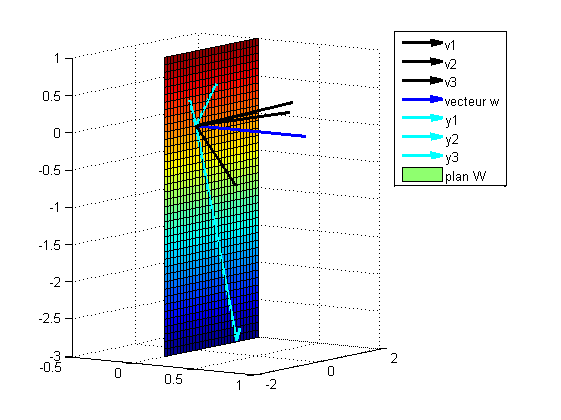
\includegraphics[width=12cm]{grapheNewton.png}\\
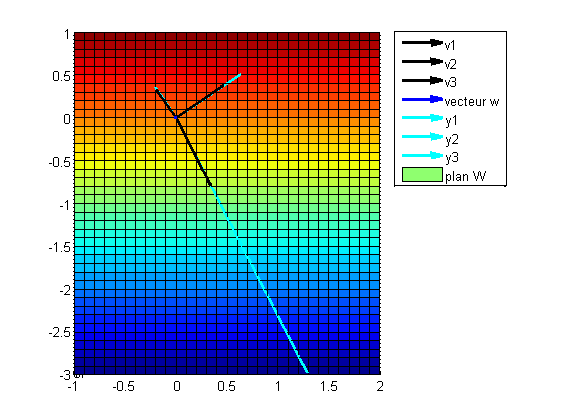
\includegraphics[width=12cm]{grapheNewton2.png}
\caption{Illustration graphique de la méthode de Newton appliquée à la fonction $G$. Le vecteur bleu est $w$, qui est fixé. La méthode va chercher un $y_1$ (resp. $y_2$ ou $y_3$) tel que la somme vectorielle $w+y_1$ soit le vecteur propre $v_1$ (resp. $v_2$ ou $v_3$).}
\label{figureNewton}
\end{figure}

Si on représente la fonction $G$ pour les matrices et vecteurs explicités ci-dessus, on obtient la figure \ref{grapheG}.

\begin{figure}
\centering
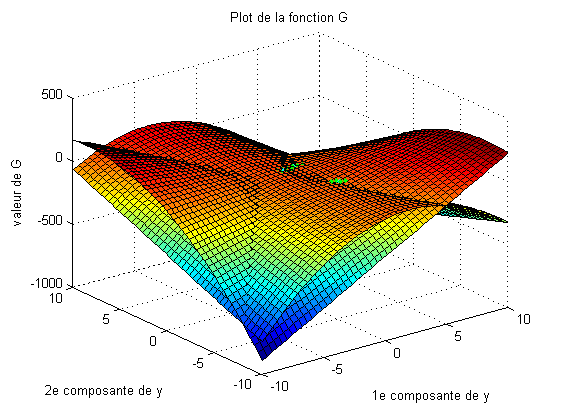
\includegraphics[width=12cm]{grapheG.png}\\
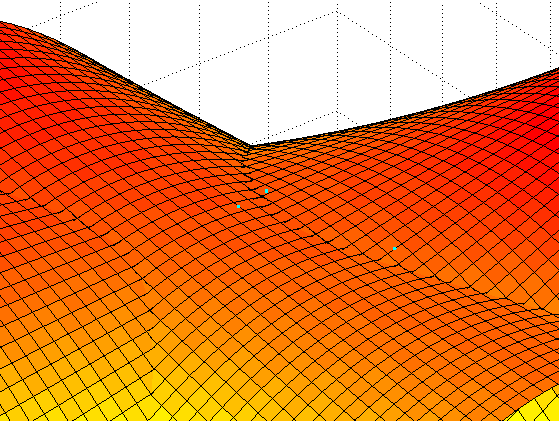
\includegraphics[width=12cm]{grapheG2.png}
\caption{Graphes de la fonction $G$. $G$ étant une fonction vectorielle à deux composantes ($G(y)=[G_1(y), G_2(y)]$), nous avons tracé les deux surfaces sur un même graphe. On cherche les points $y$ tels que $G_1(y)=G_2(y)=0$. Ces points sont tracés en vert sur les graphes ($G_1$ et $G_2$ étant ici tracés approximativement, ces points ne sont pas tous des racines mais permettent de localiser grossièrement les zones où se trouvent les vraies racines de $G$, ce qui est suffisant pour notre analyse), tandis que les points $y$ sont tracés en blanc.}
\label{grapheG}
\end{figure}
Graphiquement, la méthode de Newton, si elle converge, convergera vers le $y_i$ le plus proche de $y_0$, l'itéré de départ.\\

Regardons maintenant ce qui se passe quand $w$ est orthogonal au vecteur propre dominant, disons $v_l$. Cela signifie que $v_l$ est dans le plan $W_{\bot}$. Par conséquent, on ne peut exprimer $v_l$ par $w+W_{\bot}y$ (on peut toutefois s'en rapproche de plus en plus au fur et à mesure que $||y||$ augmente jusqu'au cas extrême où $||y|| \rightarrow \infty$).\\
Ceci n'est pas vrai que pour le vecteur propre dominant, c'est le cas pour tous vecteurs propres de $A$. Illustrons ceci par un exemple.
Soit $w = 
\begin{bmatrix}
1 \\
0\\
0.3021
\end{bmatrix} \text{ et } 
W_{\bot} =  
\begin{bmatrix}
0 & 0.2672 \\
1 & 0 \\
0 & -0.8842 
\end{bmatrix}$, A et Q ne changeant pas. On remarque que la fonction $G$ n'a plus que deux racines (cf. figure \ref{FigNewtonv1inW}).

\begin{figure}
\centering
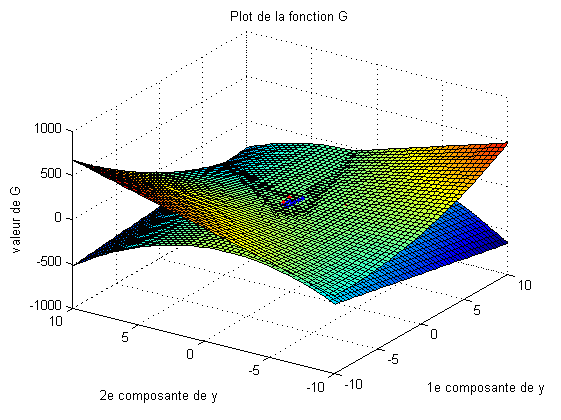
\includegraphics[width=12cm]{grapheG3.png}
\caption{Graphe de $G$ pour la même matrice $A$, mais pour $v_1 \bot w$. Deux racines, une en rouge et une bleu.}
\label{FigNewtonv1inW}
\end{figure}


\subsubsection*{Étude de la convergence}
Prenons une matrice aléatoire $A$ de taille 5 (\texttt{randn(5)}). Soit $w=[1,0,0,0,0]$ et $W_{\bot}$, son complément orthogonal. Appliquons la méthode de Newton. Les graphes de l'erreur sont donnés à la figure \ref{plor_erreur}. On observe différents comportement de la méthode de Newton. Le graphe en haut à gauche correspond au cas où Newton converge vers la solution. La droite de l'erreur à une pente qui vaut approximativement 2 ce qui correspond donc bien à une convergence d'ordre 2 (puisque on est dans un plot logarithmique, une pente de 2 signifie 2 chiffres significatif à chaque itération et donc un ordre de convergence quadratique). Remarquons que après un certain nombre d'itération, l'erreur stagne (typiquement autour des $1e-16$ ou $1e-17$) pour des raisons numériques liées à la capacité de l'ordinateur. Le graphe du haut à droite laisse entendre que la méthode a d'abord diverger puis s'est mis à converger. Le graphe du bas à gauche correspond au cas où la méthode diverge mais avec une erreur qui se stabilise après un certain temps. Et le dernier graphe correspond au cas où la méthode diverge purement et simplement.
\begin{table}
\centering
\begin{tabular}{cccc}
itération & erreur (sur $y+$) & itération & erreur\\
\end{tabular}
\end{table}  

\begin{figure}
\centering
\begin{tabular}{cc}
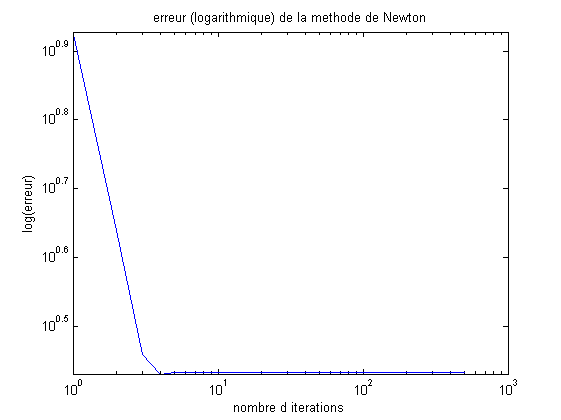
\includegraphics[width = 10cm]{erreur5.png} & 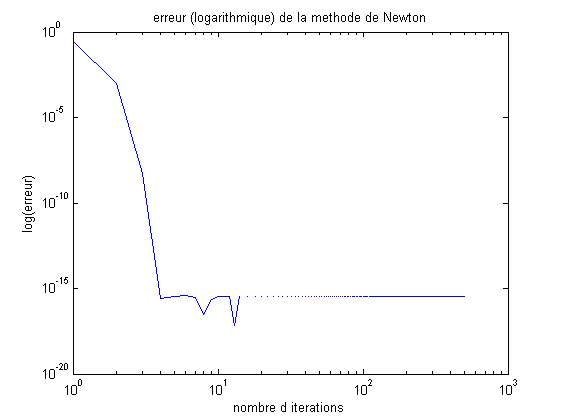
\includegraphics[width = 10cm]{erreur2.png}\\
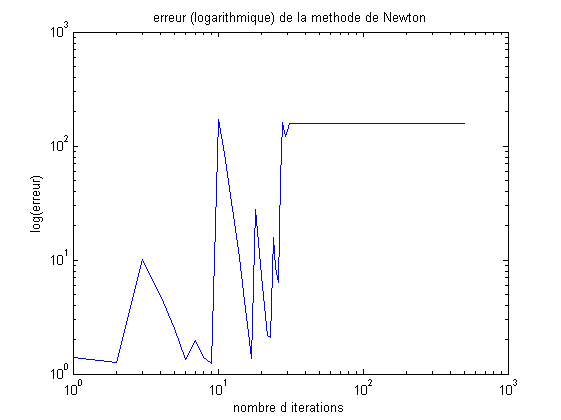
\includegraphics[width = 10cm]{erreur.png} & 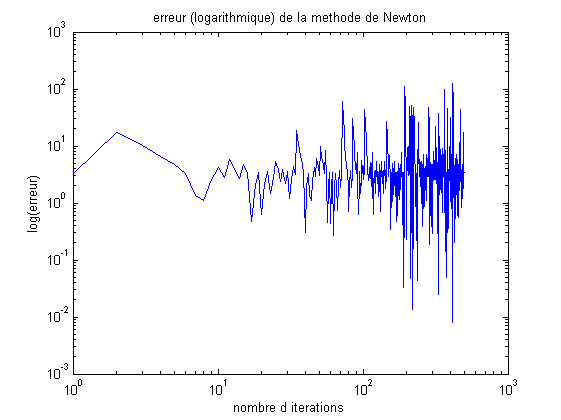
\includegraphics[width = 10cm]{erreur4.png}\\
\end{tabular}
\caption{Plot logarithmique de l'erreur à chaque itération (loglog(erreur)). }
\label{plor_erreur}
\end{figure}

\subsection*{Rayleigh symétrique}
On peut voir la méthode de Rayleigh comme une méthode de la puissance avec un "shift" variable (mis a jour à chaque itération). En d'autre mots, elle définie la méthode itérative suivante : 
$$x_{k+1} = \left(  A- \frac{x^*Ax}{x^*x}  \right)^{-1} x_k.  $$
\textbf{Proposition 4.4} Soit $A = A^*$ $ \in \mathbb{C}^{n\times n}$. L'itération du quotient de Rayleigh pour $A$ converge vers une direction propre de $A$ pour presque tout itéré initial. Lorsque la suite des itérés converge vers une direction propre, la convergence est cubique. 

Il faut maintenant préciser ce \textit{pour presque tout itéré initial}. Supposons que $A$ est diagonalisable et faisons un changement de variable afin d'exprimer $x$ dans la base formée par les vecteurs propres de $A$. Nommons le $x$ après changement de variables $x'$. Soit $Q$ la matrice dont les colonnes sont les vecteurs propres de $A$ et $D$ la matrice diagonale des valeurs propres de $A$. On utilise le théorème spectrale et le fait que $A$ et $(A-\mu I)^{-1}$ possèdent les mêmes vecteurs propres pour réécrire l'itération : 
\begin{eqnarray}
Qx_{k+1}' & = &(Q D Q^T - \frac{x_k'^* D x_k}{x_k'^* x_k})^{-1} Qx_{k}'\\
Qx_{k+1}' & = & Q(D-\frac{x_k'^* D x_k}{x_k'^* x_k})^{-1}Q^T Qx_k'\\
x_{k+1}' & = & \underbrace{(D-\frac{x_k'^* D x_k}{x_k'^* x_k})^{-1}}_{\text{matrice diagonale}} x_k'
\end{eqnarray}
Supposons qu'on souhaite converger vers le vecteur propres dominant $v_1$, autrement dit on souhaite que $lim_{k\rightarrow \infty} x_k' = [1 0 \cdots 0]^T$. Pour que cela soit possible, il faut que $x_0$ ait sa composante dans la direction $v_1$ non nulle ($x_0'^* v_1 \neq 0$). 

Vérifions maintenant de manière numérique les résultats théoriques obtenus. Prenons par exemple la matrice symétrique $A$ : 

$$ A = \left[
\begin{array}{ccc}
  2 & 4 & 6  \\
  4 & 2 & 1 \\
  6 & 1 & 2 \\
\end{array}
\right]$$

En utilisant la fonction $eigs$ de \textit{Matlab}, on sait que les valeurs propres de $A$ sont : 
   \begin{eqnarray} \label{valPropre1}
   \lambda_1 &=& 9.6965\\\label{valPropre2}
   \lambda_2 &=& 1.0796 \\\label{valPropre3}
   \lambda_3 &=& -4.7762
   \end{eqnarray}

En appliquant l'itération du quotient de Rayleigh symétrique implémentée par nos soins pour un $x_0$ tel que : 
$$ x_0 = \left[
\begin{array}{c}
  \frac{1}{\sqrt{3}}  \\
  \frac{1}{\sqrt{3}} \\
  \frac{1}{\sqrt{3}} \\
\end{array}
\right]$$
 et pour $\mu_0 = 1000$ (la valeur propre la plus "proche" est donc 9.696530) , on obtient : 
$$\begin{array}{ccc}
  itération & erreur & \mu  \\
  1 &  990.658295   & \underline{9}.341705  \\
  2 &   0.354404   &  \underline{9.696}109\\
  3 &  0.000421  & \underline{9.696530} \\
  4 &  0.000000  & \underline{9.696530} \\
\end{array}$$

Ce qui correspond bien à la théorie. En effet, à chaque itération on gagne bien 3 chiffres significatifs comme l'illustrent l'erreur (définie comme la différence entre les $\mu_k$ à chaque itération) et les chiffres soulignés qui représentent les chiffres significatifs du $\mu_k$.

On considère maintenant un itéré initial qui n'a pas de composante dans la direction du vecteur propre  

$$ v_1 = \left[
\begin{array}{c}
  0.6834  \\
   0.4317 \\
   0.5888 \\
\end{array}
\right], \text{ t.q. } Av_1 = \lambda_1 v_1,$$

par exemple  :

$$ x_0 = \left[
\begin{array}{c}
  1  \\
  0 \\
  -1.1606\\
\end{array}
\right]$$

Lorsqu'on applique l'itération, on ne converge effectivement plus vers $\lambda_1$ mais vers $\lambda_3$. Le \textit{pour presque tout itéré initial} est donc confirmé.


La figure \ref{fig:RaySym} illustre les valeurs propres (sur l'axe des z, cf. \ref{valPropre1}, \ref{valPropre2} et \ref{valPropre3} pour leur valeur) vers lesquelles l'itération converge pour différents vecteurs propres initiaux $x_0$ (représentés par les points 1, 2 ou 3 sur l'axe des x) et pour différents $\mu$ initiaux (de -10 à 10 sur l'axe des y). Le point 1 de l'axe des x représente le vecteur initial le plus proche du vecteur propre relatif à la valeur propre $\lambda_1$, le deuxième à $\lambda_2$ et le troisième à $\lambda_3$. On constate que lorsque $\mu$ est très proche d'une valeur propre, on aura tendance à converger vers cette valeur, par contre si on s'éloigne on convergera vers la valeur propre pour laquelle le vecteur propre est le plus proche du vecteur initial\footnote{On constate qu'une valeur propre est incohérente par rapport aux autres, ceci est du au fait que, lorsqu'on applique l'algorithme, si on choisit mal le $\mu$ et $x_0$ il est possible qu'après un certain nombre d'itération, on tombe par hasard sur un $\mu$ qui sera identique à l'itération $k-1$ et $k$. Or vu que nous avons défini notre erreur comme la différence des $\mu$, certaines fois l'algorithme s'arrête à cause d'une égalité fortuite  }. 

\begin{figure}
  \centering
  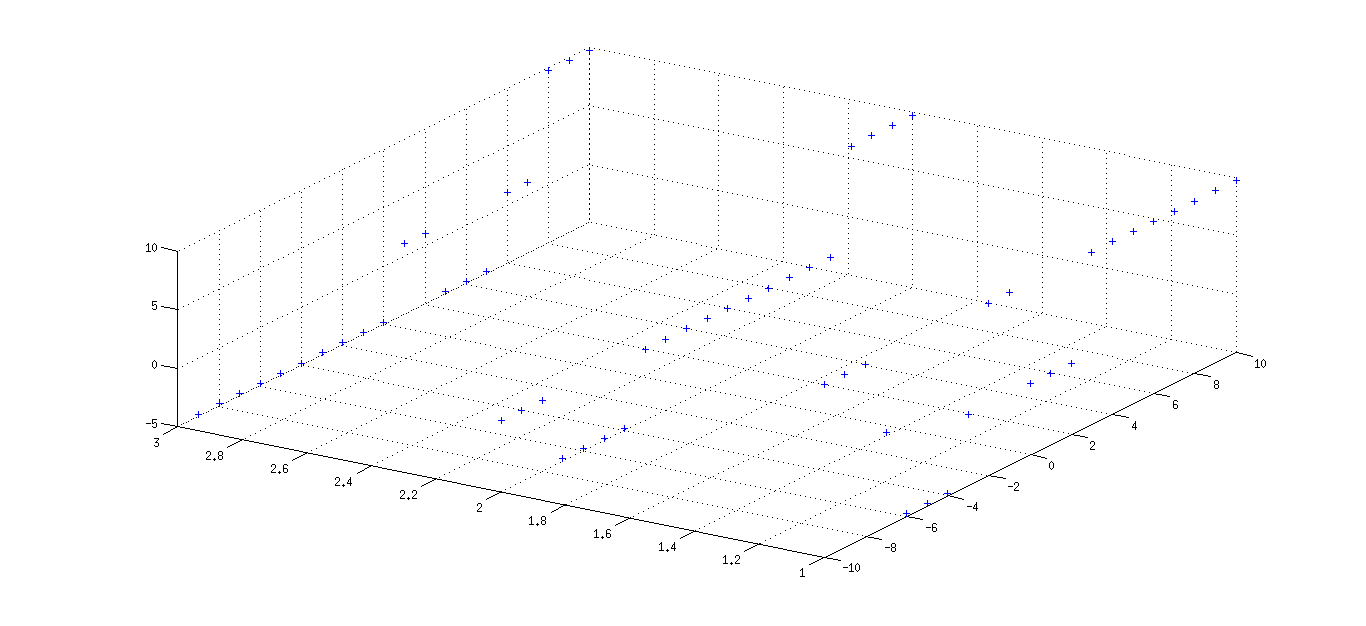
\includegraphics[width=15cm]{RaySym.png}
  \caption{Graphe représentant les valeurs propres vers lesquelles on converge pour différents $x_0$ et $\mu$}
  \label{fig:RaySym}
\end{figure}

\subsection*{Rayleigh asymétrique}

	Tout d'abord assurons nous que l'itération asymétrique du quotient de Rayleigh converge bien dans le cas où l'on prend $x_0$ et $y_0$ identiques et que l'on retombe donc sur l'itération symétrique. On constate aisément que l'on retombe sur les mêmes résultats, c'est juste sensiblement plus lent vu qu'on fait deux fois certains calculs. 
	
	Au niveau de la vitesse de convergence, on reste dans le même ordre de grandeur que pour Rayleigh symétrique si on choisit des vecteurs à plus ou moins même distance relative d'un vecteur propre. \textbf{si il y en a 1 qui est chaud faire un petit tableau, en soit ca a pas full intéret juste du remplissage }
	MAIS C EST UN AVANTAGE SI ON  SAIT PAS TROP OU ALLER DE POUVOIR CHOISIR 2 VECT INITIAUX ! (\textbf{A faire, la on pourrait peut etre un peu blabla sur le fait que on peut peut etre taper plus au pif que pour sym})
	
	Si on considère un des deux vecteurs initiaux orthogonal à un vecteur propre. (\textbf{A faire, ca bug comme pour sym.})
	
	
	Enfin, considérons comme pour la méthode de Rayleigh symétrique, différents vecteurs initiaux ainsi que différents $\rho_0$. (\textbf{A commenter, meme conclusions que pour sym rien d'hors du commun})
	
	
	
\begin{figure}
  \centering
  \begin{subfigure}[b]{0.85\textwidth}
    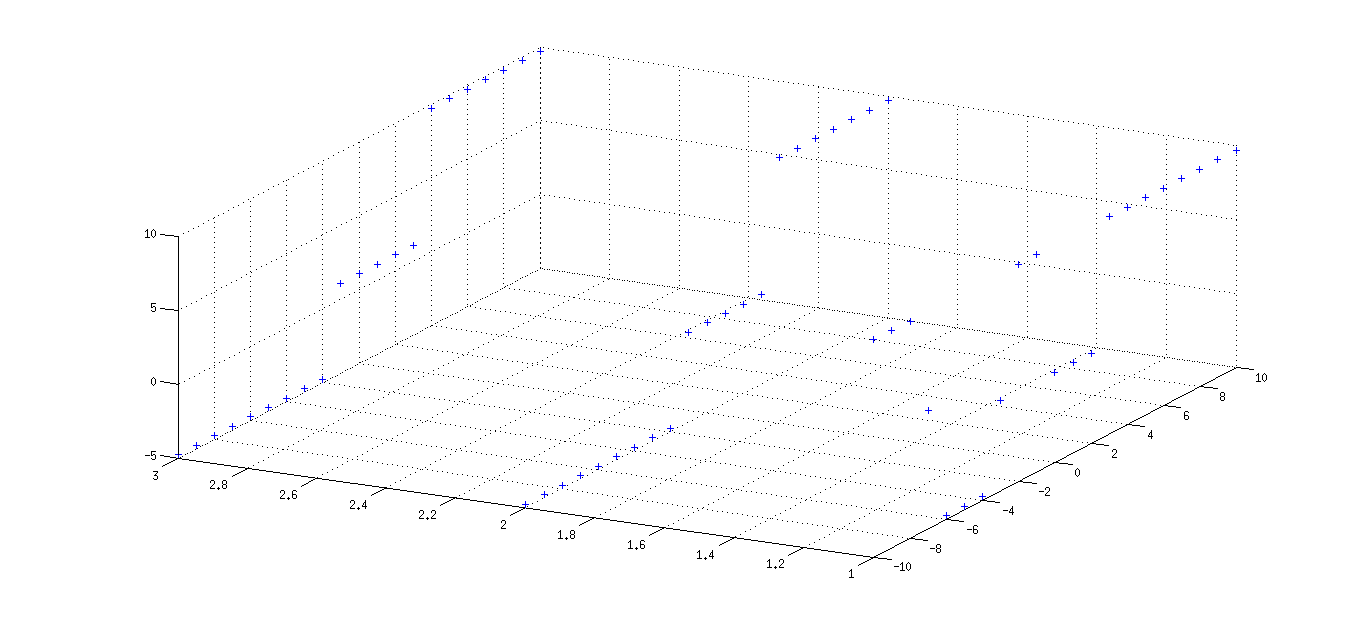
\includegraphics[width=\textwidth]{RayAsym1.png}
    \caption{Pour un vecteur initial proche du premier vecteur propre.}
    \label{fig:a4}
  \end{subfigure}%
  
  %add desired spacing between images, e. g. ~, \quad, \qquad etc.
  %(or a blank line to force the subfigure onto a new line)
  \begin{subfigure}[b]{0.85\textwidth}
    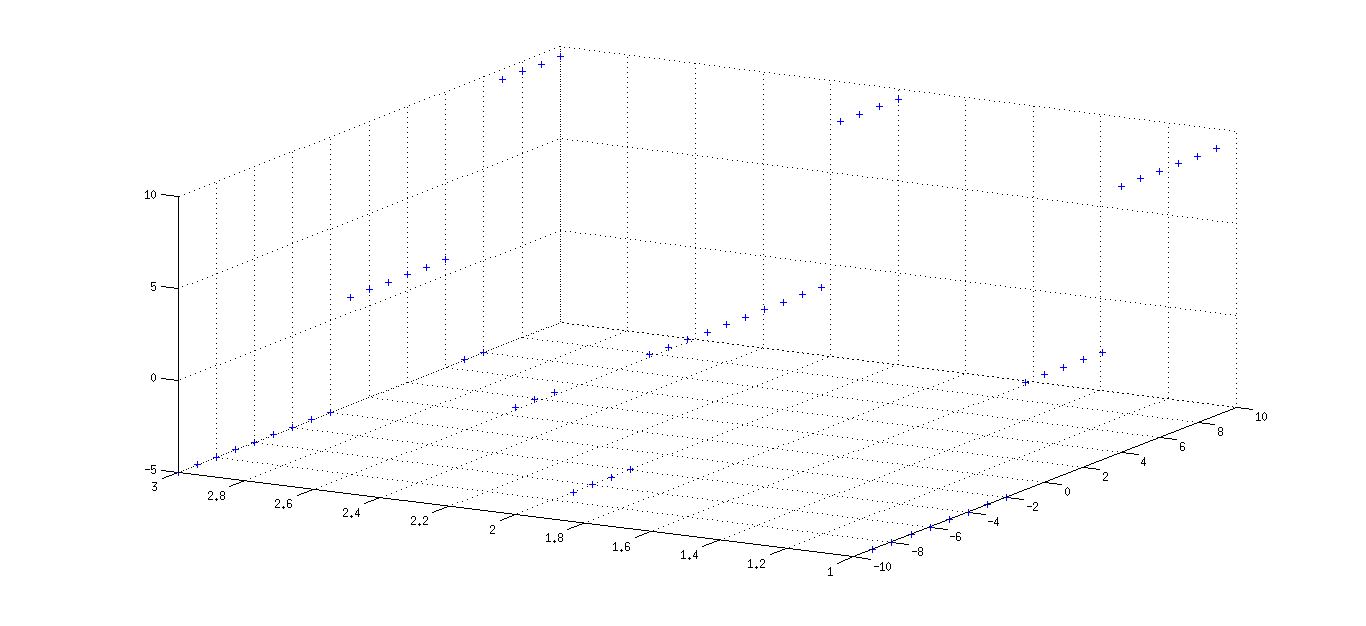
\includegraphics[width=\textwidth]{RayAsym2.png}
    \caption{Pour un vecteur initial proche du second vecteur propre.}
    \label{fig:a45}
  \end{subfigure}%
  
  \begin{subfigure}[b]{0.85\textwidth}
    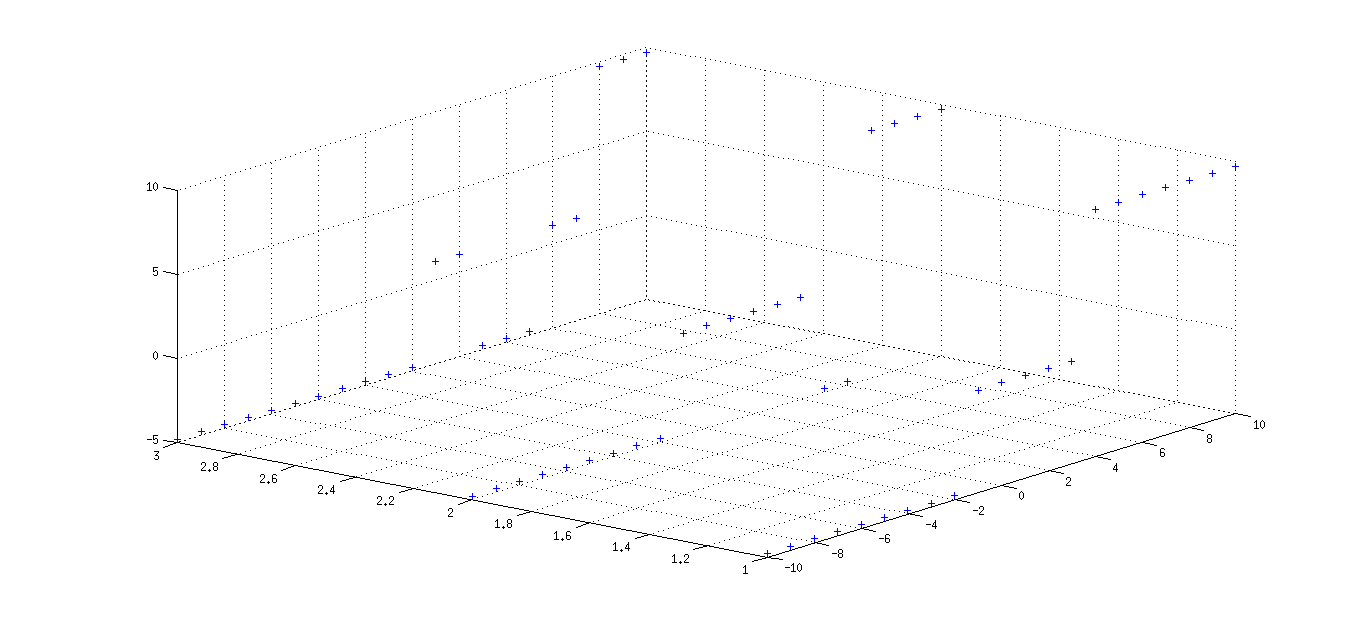
\includegraphics[width=\textwidth]{RayAsym3.png}
    \caption{Pour un vecteur initial proche du troisième vecteur propre.}
    \label{fig:a5}
  \end{subfigure}
  \caption{Valeurs propres vers lesquelles l'algorithme de l'itération asymétrique du quotient de Rayleigh converge. Les 3 graphes représentent chacun d'eux un $x_0$ différent pour lesquels on a fait varier le $y_0$ et le $\rho_0$.}\label{fig:adiff}
\end{figure}	
